\subsection{Moving a Cube}
Before moving a cube, the cube must first be rotated to a different face.
This rotation is entirely based on whether the die rolled was even or odd.
After the cube has been rotated, it is then moved the indicated number of spaces orthogonally in any direction on the board, though never crossing back over the starting line.

Cubes also cannot pass over each other.

\paragraph{If the Die Shows Even} The cube's face value is increased to the next available value
$$1 \to 8 \to 16 \to 24 \to 32 \to 40 \to 1$$
\paragraph{If the Die Shows Odd} The cube's face value is decreased to the previous value
$$40 \to 32 \to 24 \to 16 \to 8 \to 1 \to 40$$

\note In either case, a roll-over happens if a player tries to increase or decrease past the highest or lowest value respectively.

\begin{figure}[!h]
    \centering
    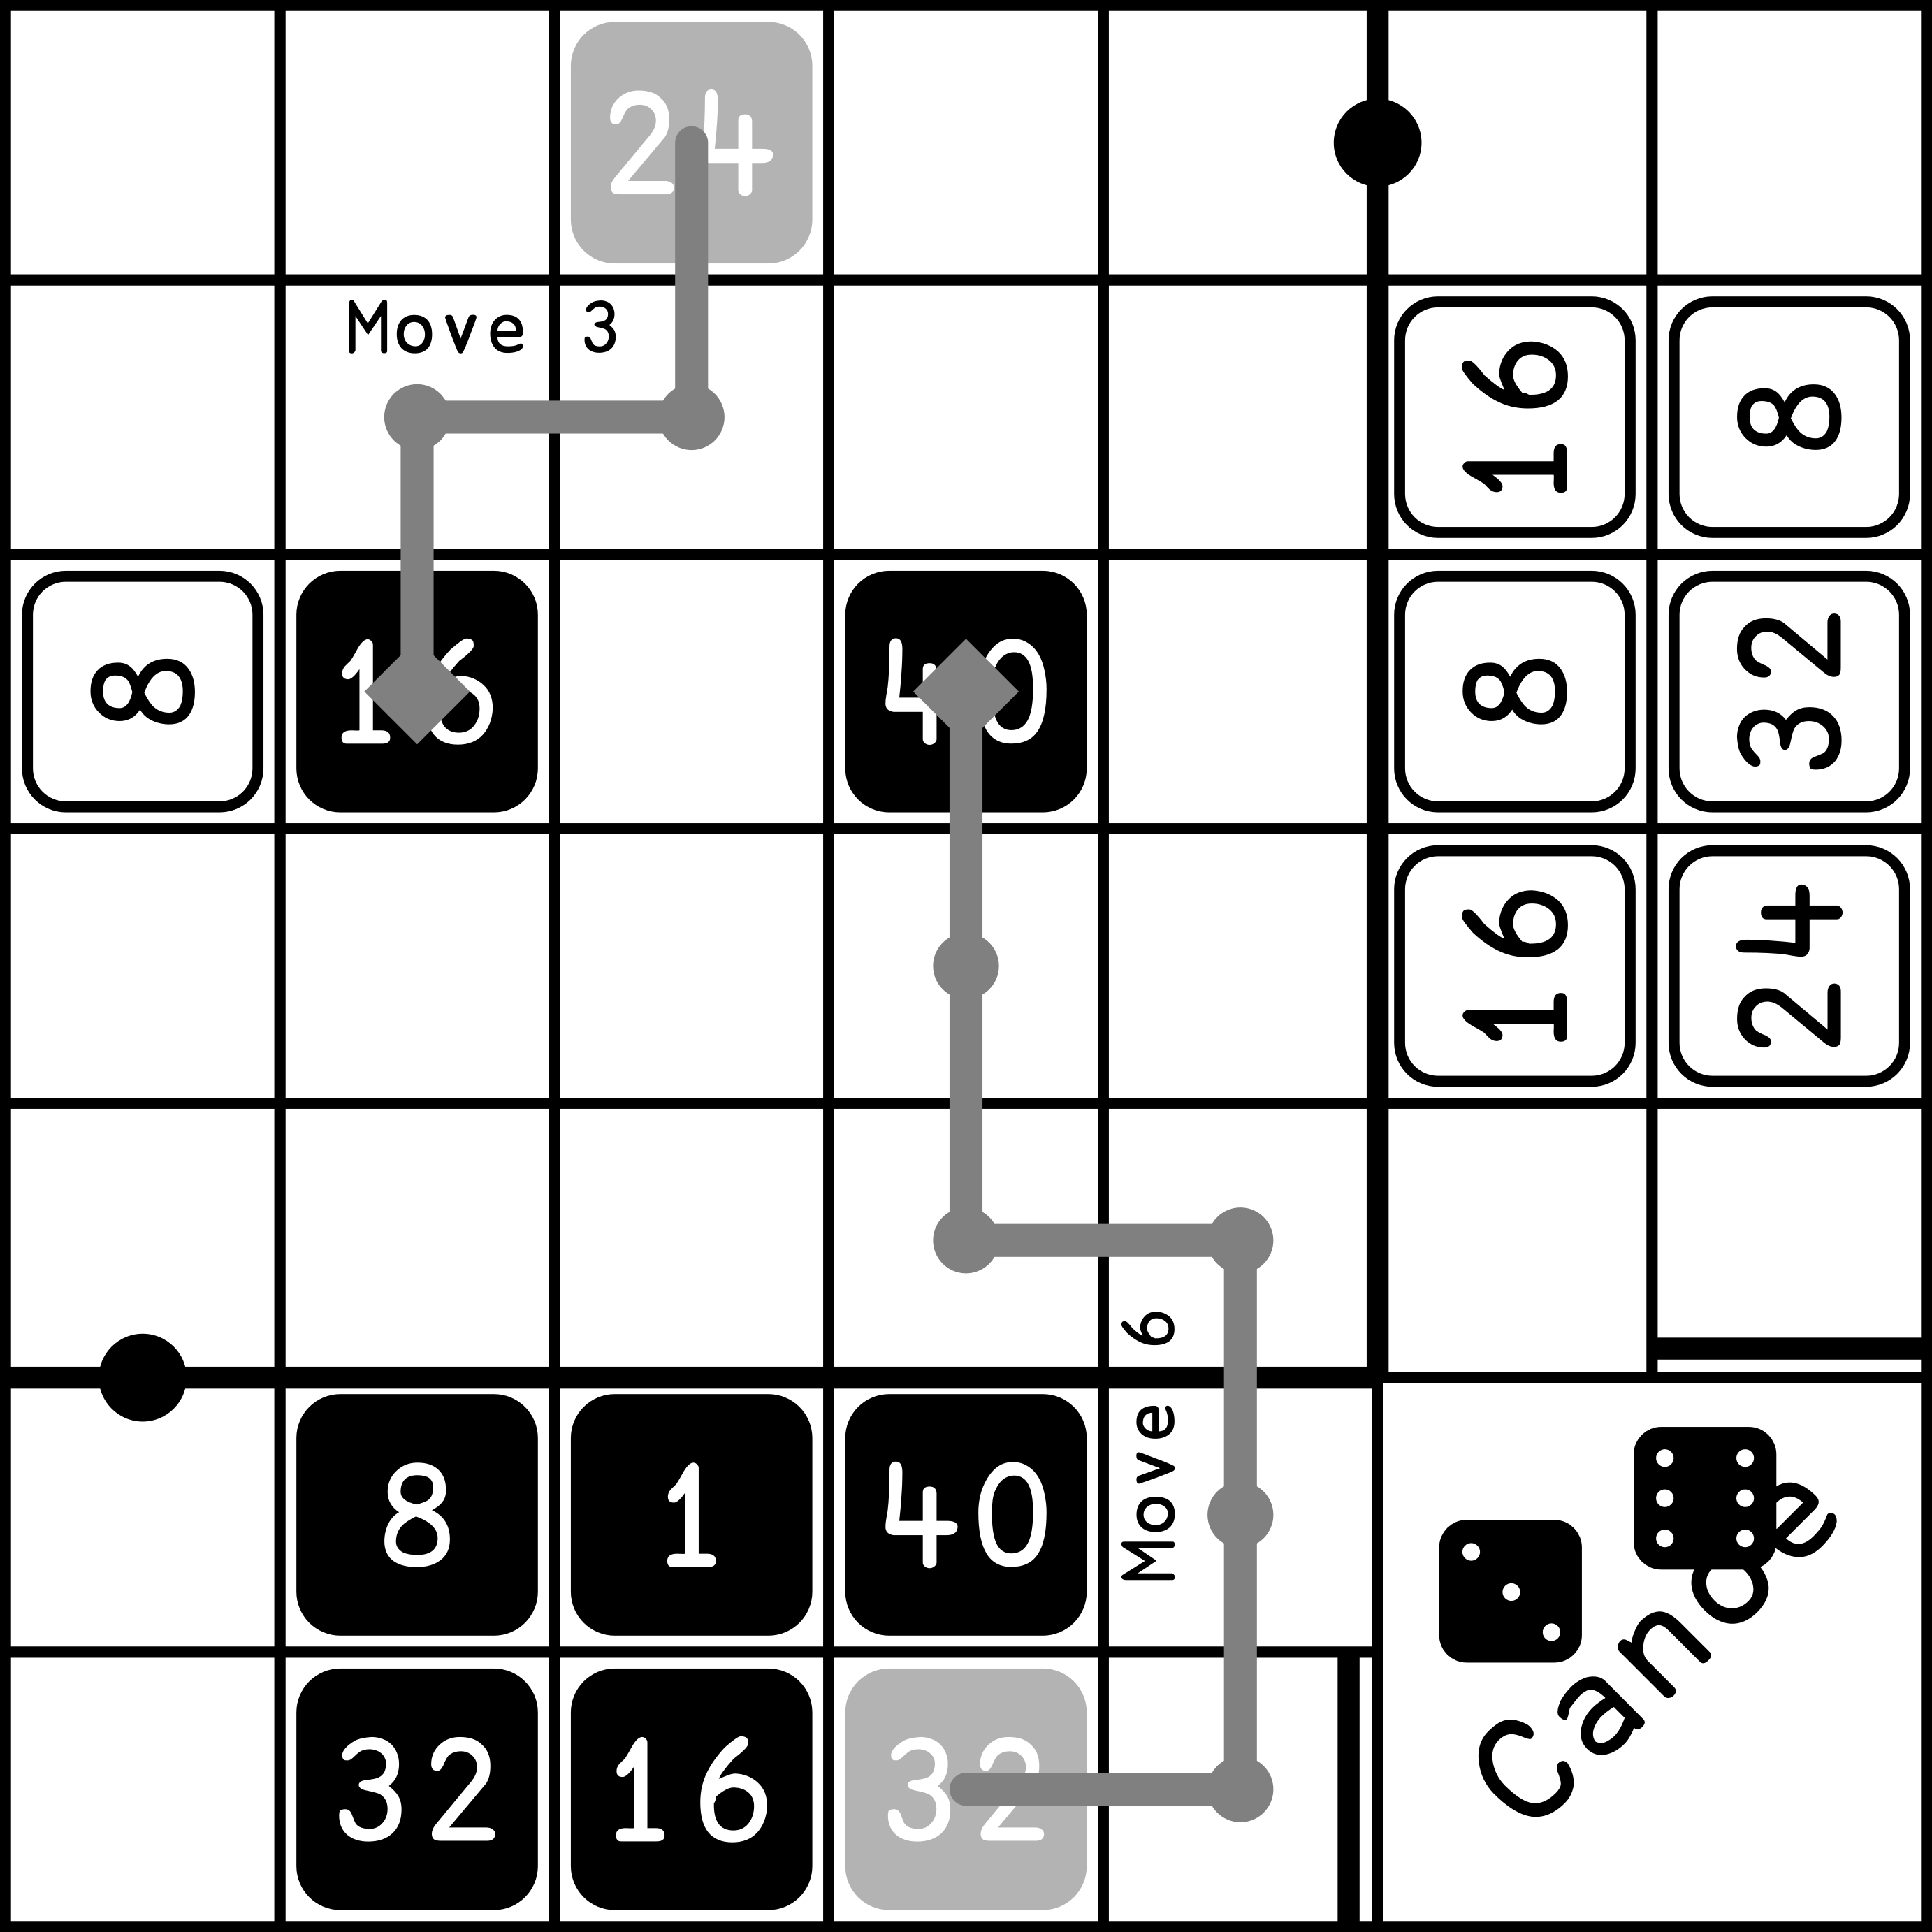
\includegraphics[width=8cm]{../graphics/movement}
    \caption{Example Move}
    \label{fig:move}
\end{figure}

\example In Figure~\ref{fig:move}, Billy rolled a \epsdice{6} and a \epsdice{3}, and has decided to move his 24 cube three spaces. 
He first rotates the cube so it shows 16 before moving it those three spaces. 
Next he wants to move his 32 cube six spaces, he first rotates the cube so it instead shows 40, and then moves it six spaces.

\subsubsection{Stymie}
In the event that a player has exactly two cubes left, and both share the same number and are adjacent or an even number of spaces apart, then that player may choose to call ``Stymie'' and only roll one die on their turn.